\tableofcontents

\newpage

\section{Задание}
Синтезировать цикл исполнения для выданных преподавателем команд. Разработать тестовые программы, которые проверяют каждую из синтезированных команд. Загрузить в микропрограммную память БЭВМ циклы исполнения синтезированных команд, загрузить в основную память БЭВМ тестовые программы. Проверить и отладить разработанные тестовые программы и микропрограммы.
\begin{figure}[H]
\centering
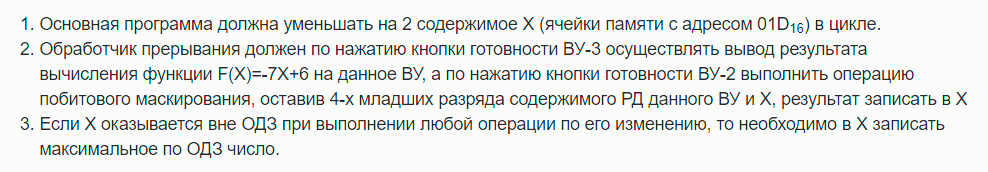
\includegraphics[scale=0.52]{task}
\label{pic:task}
\end{figure}

\section{Текст синтезированной микропрограммы}
\begin{center}
\begin{tabular}{|c|c|l|}
\hline
\textbf{Адрес МП} & \textbf{Микрокоманда} & \textbf{Действие}\\
\hline
3D & 81E1104002 & if CR(12) = 1 then GOTO E1\\
\hline
E1 & 80E4011040 & if PS(C) = 0 then GOTO E4\\
E2 & 0001009411 & AC + DR + 1 $\rightarrow$ DR\\
E3 & 80E5101040 & GOTO E5\\
E4 & 0001009011 & AC + DR $\rightarrow$ DR\\
E5 & 0200000000 & DR $\rightarrow$ MEM(AR)\\
E6 & 80C4101040 & GOTO INT @ C4\\
\hline
\end{tabular}
\end{center}

\section{Текст тестовой программы}
\begin{center}
\begin{tabular}{c}
\begin{lstlisting}[basicstyle=\ttfamily]
	ORG 0xF9
TR1:	WORD ?
TR2:	WORD ?
TR3:	WORD ?
RES:	WORD 1

START:	CALL T1
	ST TR1
	BNE N2
	ST RES
N2:	CALL T2
	ST TR2
	BNE N3
	ST RES
N3:	CALL T3
	ST TR3
	BNE EN
	ST RES
EN:	HLT

A1:	WORD 0x1
B1:	WORD 0x2
R1:	WORD 0x3
T1:	LD A1
	WORD 0x9EFC
	LD B1
	CMP R1
	BNE WR
	BR COR
\end{lstlisting}
\end{tabular}
\end{center}


\begin{center}
\begin{tabular}{c}
\begin{lstlisting}[basicstyle=\ttfamily]
A2:	WORD 0x1
B2:	WORD 0x2
R2:	WORD 0x4
T2:	CLC
	CMC
	LD A1
	WORD 0x9EFC
	LD B1
	CMP R1
	BNE WR
	BR COR

A3:	WORD 0x1
B3:	WORD 0x2
T3:	CLC
	CMC
	LD A1
	WORD 0x9EFC
	BCC WR
	BR COR

COR:	LD #1
	RET
WR:	LD #0
	RET
\end{lstlisting}
\end{tabular}
\end{center}

\section{Таблица трассировки микрокоманд}
\begin{center}
\begin{tabular}{|c|c|c|c|c|c|c|c|c|c|}
\hline
\multirow{2}{*}{\makecell{\textbf{МР до}\\\textbf{выборки МК}}} &
\multicolumn{9}{c|}{\textbf{\makecell{\textbf{Содердимое памяти и регистров процессора}\\\textbf{после выборки и исполнения микрокоманды}}}}\\
\cline{2-10}
& MR & IP & CR & AR & DR & BR & AC & NZVC & МР (СчМК)\\
\hline
28 & 813C804002 & 10F & 9EFC & 10B & 0002 & FFFC & 0001 & 0000 & 3C\\
\hline
3C & 8143204002 & 10F & 9EFC & 10B & 0002 & FFFC & 0001 & 0000 & 3D\\
\hline
3D & 81E1104002 & 10F & 9EFC & 10B & 0002 & FFFC & 0001 & 0000 & E1\\
\hline
E1 & 80E4011040 & 10F & 9EFC & 10B & 0002 & FFFC & 0001 & 0000 & E4\\
\hline
E4 & 0001009011 & 10F & 9EFC & 10B & 0003 & FFFC & 0001 & 0000 & E5\\
\hline
E5 & 0200000000 & 10F & 9EFC & 10B & 0003 & FFFC & 0001 & 0000 & E6\\
\hline
E6 & 80C4101040 & 10F & 9EFC & 10B & 0003 & FFFC & 0001 & 0000 & C4\\
\hline
\end{tabular}
\end{center}

\section{Методика проверки команды}
\begin{enumerate}
\item Занести микрокод в микропрограммную память, а тестовую программу в основную память БЭВМ.
\item Запустить программу с адреса 0x0FD в режиме `Работа'.
\item Дождаться останова БЭВМ.
\item Проверить значение ячейки памяти RES (0x0FC) с помощью пультовой операции `Чтение'.
\item Если там записана `1', то все тесты успешно пройдены. Если `0', проверить, какой тест не пройден, считывая значения ячеек TR1 (0x0F9) -- TR3 (0x0FB) по аналогии.\\

T1: Проверка корректной записи результата\\
T2: Проверка использования флага переноса\\
T3: Проверка сохранения состояния флага C
\end{enumerate}

\section{Вывод}
В ходе выполнения данной лабораторной работы я познакомился с работой МПУ в БЭВМ, видами микрокоманд и внутренней работой некоторых элементов БЭВМ. Эти знания пригодятся мне для понимания работы современных ЭВМ.
